\subsection{Deadlock Detection}
\label{sec:dld}
We take advantage of the rich collection of information about the dynamic behavior of within ECT to automatically identify whether one or more goroutines have been leaked after program termination.

Upon program termination, we construct a goroutine tree (figure \ref{fig:gtree}) of application goroutines by replaying through the execution ECT.
%
In the goroutine tree, parents are the goroutines that children are created from within them. Each node of the tree contains information about the goroutine creation site, the resources that it holds at each execution point and the final executed event right before program termination.
%
In the lifetime of a program, the runtime system creates new goroutines or pick from the pool of dead goroutines to perform various tasks such as bootstrapping the program, garbage marking and sweeping, and tracing.
%
\goat also adds extra goroutine to \textit{watch} the main goroutine in case of blockage of the main goroutine.
%
These extra goroutines are captured in the tracing but we are not interested in studying them as our main focus is the main application (or test) and all application-level goroutines.
%
By checking the stack of creation location, \goat prune the goroutine and only keep the \textit{application-level} goroutines.
%
We say a goroutine is an application-level goroutine if it is the main goroutine (that executes the main function) or it has all of the following conditions:
1) its ancestor is the main goroutine,
2) it is not a Go runtime system goroutine, and
3) it is not a tracer goroutine.
Such distinguishment between goroutines is essential to define the boundaries of the application and the underlying system.



\begin{figure}[]

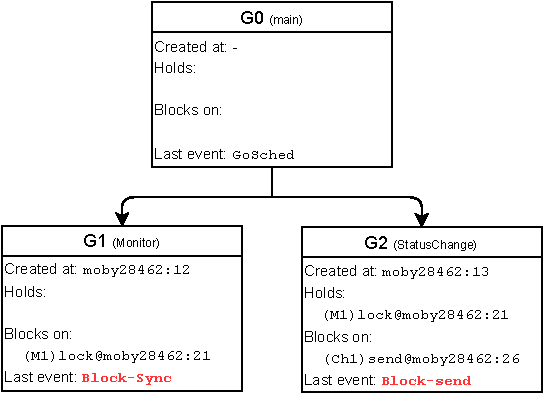
\includegraphics[width=0.9\linewidth]{figs/gtree.pdf}
%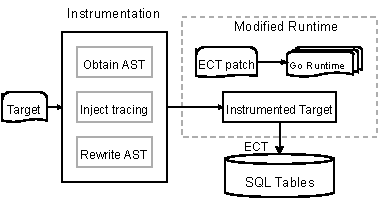
\includegraphics[]{figs/overview.png}
%\includegraphics[]{figs/overv}
\label{fig:gtree}
\caption{Goroutine tree of leaky execution of listing \ref{listing:moby28462}}
\end{figure}

Upon program termination, we construct a goroutine tree (figure \ref{fig:gtree}) of application goroutines by replaying through the execution ECT.
%
In addition to the parent/children relation of goroutines, nodes of the goroutine tree contains information about the goroutine creation site, the resources that it holds at each execution point and the final executed event right before program termination.
%
If tracing is enabled, every application goroutine invokes the tracer to capture $GoEnd$ before finishing its execution and exit (change status from \textit{grunnable} to \textit{gdead})\cite{goexit-line-of-code}.
%
Before the main function returns (\ie exits), it calls the scheduler (through \texttt{runtime.Gosched()} invocation which captures $GoSched$ event) to hand over the control to the root goroutine to finish up program execution.
%
Since we instrument the application to call \texttt{runtime.traceStop} to stop tracing when main returns, $GoSched$ would be the last event captured for the main goroutine if it returns succesfully.
%
We call an execution \textbf{successful}, if below conditions hold
\begin{description}
  \item (1) all goroutines spawned in the main goroutine has $GoEnd$ as their final event
  \item (2) the final event of the main goroutine is $GoSched$ with \texttt{runtime.traceStop} on top of its stack.
\end{description}


If either of above conditions does not satisfy after program execution, a \textbf{deadlock} happens because it shows that there are one or more goroutine that did not reach its final state. In other words:

if \texttt{finalEvent(}ECT.G$_{main}$\texttt{)} $\neq GoSched \Rightarrow Global Deadlock (GDL)$
else
  for ECT.G$_{appi}$ in application-level goroutines  :
    if \texttt{finalEvent(}ECT.G$_{main}$\texttt{)} $\neq GoSched \Rightarrow Partial Deadlock (PDL)$

    else:
    $Successful$

%
Other execution models such as figure \ref{fig:execVis} are also constructible when replaying the execution ECT.
%
\stcmt{I want to say that middlewares like DiffTrace and GOAT are helpful for human debuggers, because at the end of the day, nothing can be done fully automatically}
Human debuggers can use such models to review program execution and compare their expectations with actual behavior.
%
\stcmtside{future work}
Moreover, online or offline verifiers can take ECT as input and construct logical models to verify the program execution.
%


\begin{figure}[]
\centering

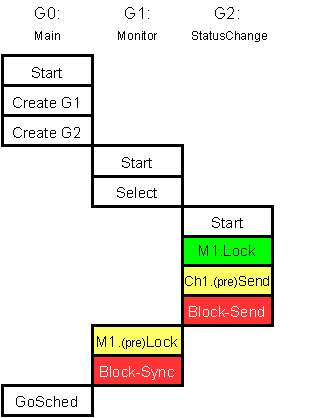
\includegraphics[width=0.6\linewidth]{figs/execVis.pdf}
\caption{Execution visualization of leaky interleaving in \ref{listing:moby28462} by replaying ECT}
\label{fig:execVis}
\end{figure}

\begin{figure}
\centering
  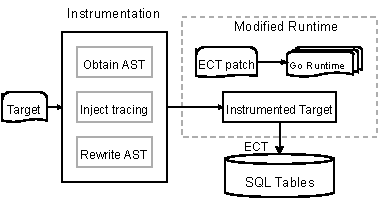
\includegraphics[width=.95\linewidth]{figs/overview.pdf}
  \caption{Framework Overview (NEED TO UPDATE)}
  \label{fig:overview}
\end{figure}

\subsection{Accelerating Bug Exposure}
\label{sec:critical}
As we have shown in figure \ref{fig:rare_bugs}, there are cases that the deadlock is hidden in the interleaving space.
%
It is proved that context-switches before synchronization/serialization operations in concurrent programs increases the probability of finding rare concurrent bugs \cite{burckhardt-depthBug-asplos10}.
%
For example, a rare context-switch right after the select statement in line \ref{bugListing:Monitor_select} causes the lock operation on mutex $m$ in line \ref{bugListing:Monitor_case_def_lock} of goroutine \texttt{Monitor} to \textit{block} goroutine \texttt{StatusChange} on locking $m$ in line \ref{bugListing:statChange_lock} and causing a deadlock.
%
Concurrency primitive usages are the \textit{critical points} in the program because their behavior directly impacts the blocking behavior of Go programs.
%
In \goat, we identify the usage of concurrency primitives as the critical points of the program before which a context-switch increases the probablity of manifesting a hidden bug that might not occur during conventional or stress testing.
%These critical points are interesting to study application correctness because 1)their behavior depends on the state of other goroutines at each execution step, 2) investigating their behavior and interaction with other goroutines is the key to debug the program behavior, 2) a contex-switch before their execution might change the operation behavior, and consequently the whole program behavior.
%
%
We define \textit{concurrency usage} (CU) as a triple of $<f,l,k>$ where $f$ is the file name, $l$ is the line number and $k$ is the kind of concurrency primitive used in the code location.
Kind $k\in$ \texttt{Channel} $\cup$ \texttt{Sync} $\cup$ \texttt{Go}:
\begin{itemize}
  \item \texttt{Channel} = \{\texttt{send}, \texttt{receive}, \texttt{close}\}
  \item \texttt{Sync} = \{\texttt{lock}, \texttt{unlock}, \texttt{wait}, \texttt{add}, \texttt{done}, \texttt{signal}, \texttt{broadcast}\}
  \item \texttt{Go} = \{\texttt{go}, \texttt{select}, \texttt{range}\}
\end{itemize}

The first column of table \ref{tab:moby_cov_table} shows the critical points extracted from program in listing \ref{listing:moby28462}.
%
We identify CU points by parsing the abstract syntax tree (AST) of the target source using Go AST package \cite{go-package-ast}.

CU points are passed to the instrumentation phase of \goat to inject scheduler perturbation handlers before these points.
%
%
%
% Through statically traversing the AST of any target package (e.g., files of the “main” package), goat gathers a set of line numbers where concurrency functions are used. These points (aka critical points) are the points where a context switch might drastically change the concurrency behavior of the program and trigger an undiscovered bug. Here are the AST nodes that represent a critical point:
% Go: ast.Node GoStmt   (example: go func() // spawning a new goroutine)
% Send: ast.Node SendStmt     (example: channel <- x)
% Recv: ast.Node UniExprStmt(op=”<-”) (example:  <- channel)
% Mutex, WaitGroup, CondVars: ast.Node CallExpr (example: xxx.Lock())
% Xxx.Lock()
% Xxx.Unlock()
% Xxx.Add()
% Xxx.Wait()
% Xxx.Signal()
% Xxx.Broadcast()
% Careful adjustment is required for Select and Range statements that have send/recv as their children in the AST.

\subsection{Instrumentation}
\label{sec:instrument}
\stcmt{below is the raw text that I wrote for instrumentation. I will complete it}
We equip target applications with \goat functionalities by automatically injecting
Identifying “critical points”:
Instrumentation: goat inject goat\_handler() calls before the critical point nodes. Goat\_handler() can be a call to any desired scheduler-manipulator. For instance, currently it calls an external function that randomly and boundedly yield to all other runnable goroutines (i.e., call gosched()). It gives us the flexibility to experiment different kinds of random and systematic (e.g., coverage-guided) scheduler-manipulation from an external function and environment variables without touching goat or goatlib API. In addition to critical points, goat adds four more line to the beginning of main function:
Import goat
goat\_done := goat.Start() // Start() initializes goat and starts tracing. It also creates and returns a channel for signaling the Stop()
go goat.Watch(goat\_done) // spawns a new goroutine as a watcher for liveness of the program (in case of global deadlocks or infinite loop). Watch() either receives from done and performs : goat\_done <- true, or timeouts and stop tracing, and terminates.
defer goat.Stop(goat\_done) // after the main ends, Stop() is called to send a value to the watcher goroutine and signaling that the program is finished. Then it waits to receive the ack from watcher, then stops tracing and terminates.
Trace collection: Currently, goat can collect a plain ECT from the native execution and also ECTs from executions with manipulated scheduler.

\subsection{Evaluation}

\stcmt{Experimental methodology - GoKer - Two main figures, one table I will add}
\begin{itemize}
  \item Figure \ref{fig:detection} : How \textbf{WELL} we detected bugs comparing to others
  \item Figure \ref{fig:runs} : How \textbf{SOON} we detected bugs comparing to others
\end{itemize}



\begin{figure}
\centering
  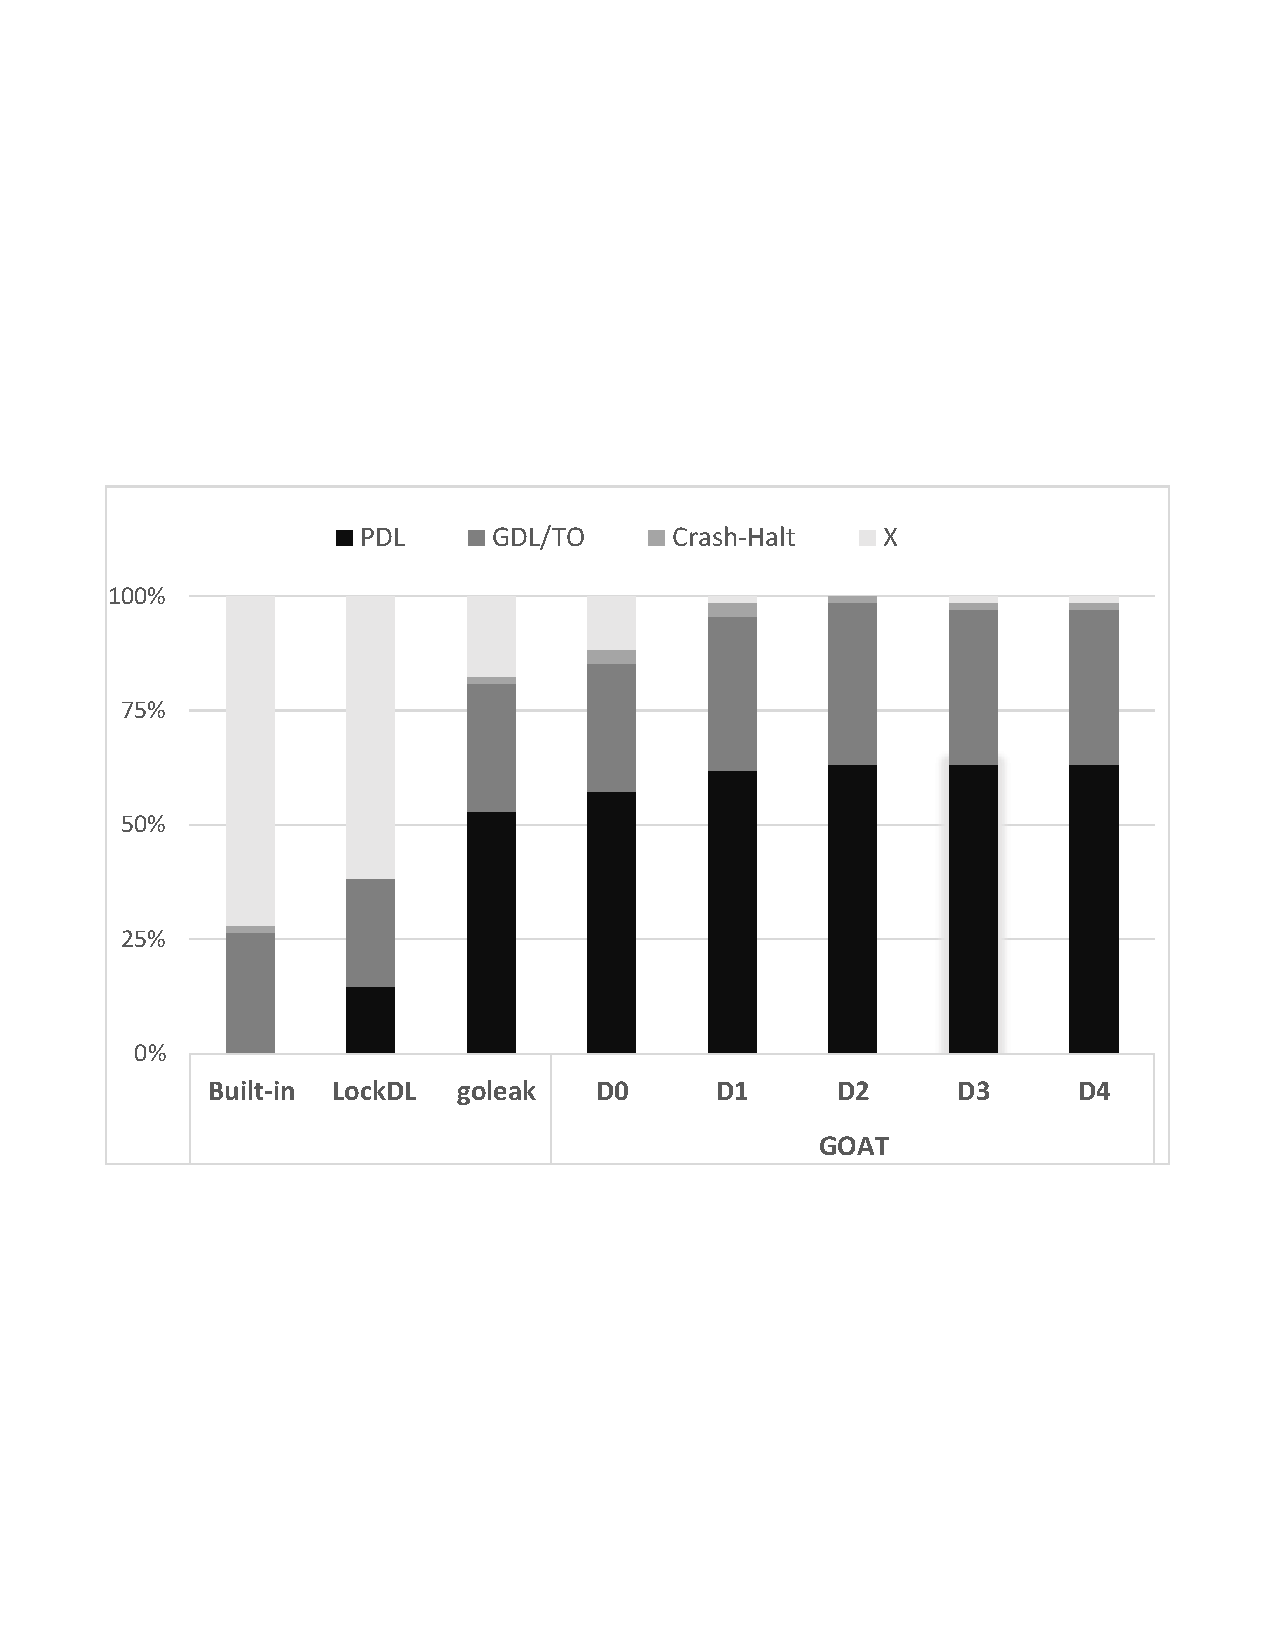
\includegraphics[width=.95\linewidth]{figs/P4_detections.pdf}
  \caption{Distribution of detected bugs by built-in deadlock detector (BUILTINDL), LockDL, GoLeak, and GOAT different d. (over 1000 runs). pdl: partial deadlock, gdl: global deadlock, crash/halt: causes the program to crash or halt on detection, x: nothing is detected }
  \label{fig:detection}
\end{figure}


\begin{figure}
\centering
  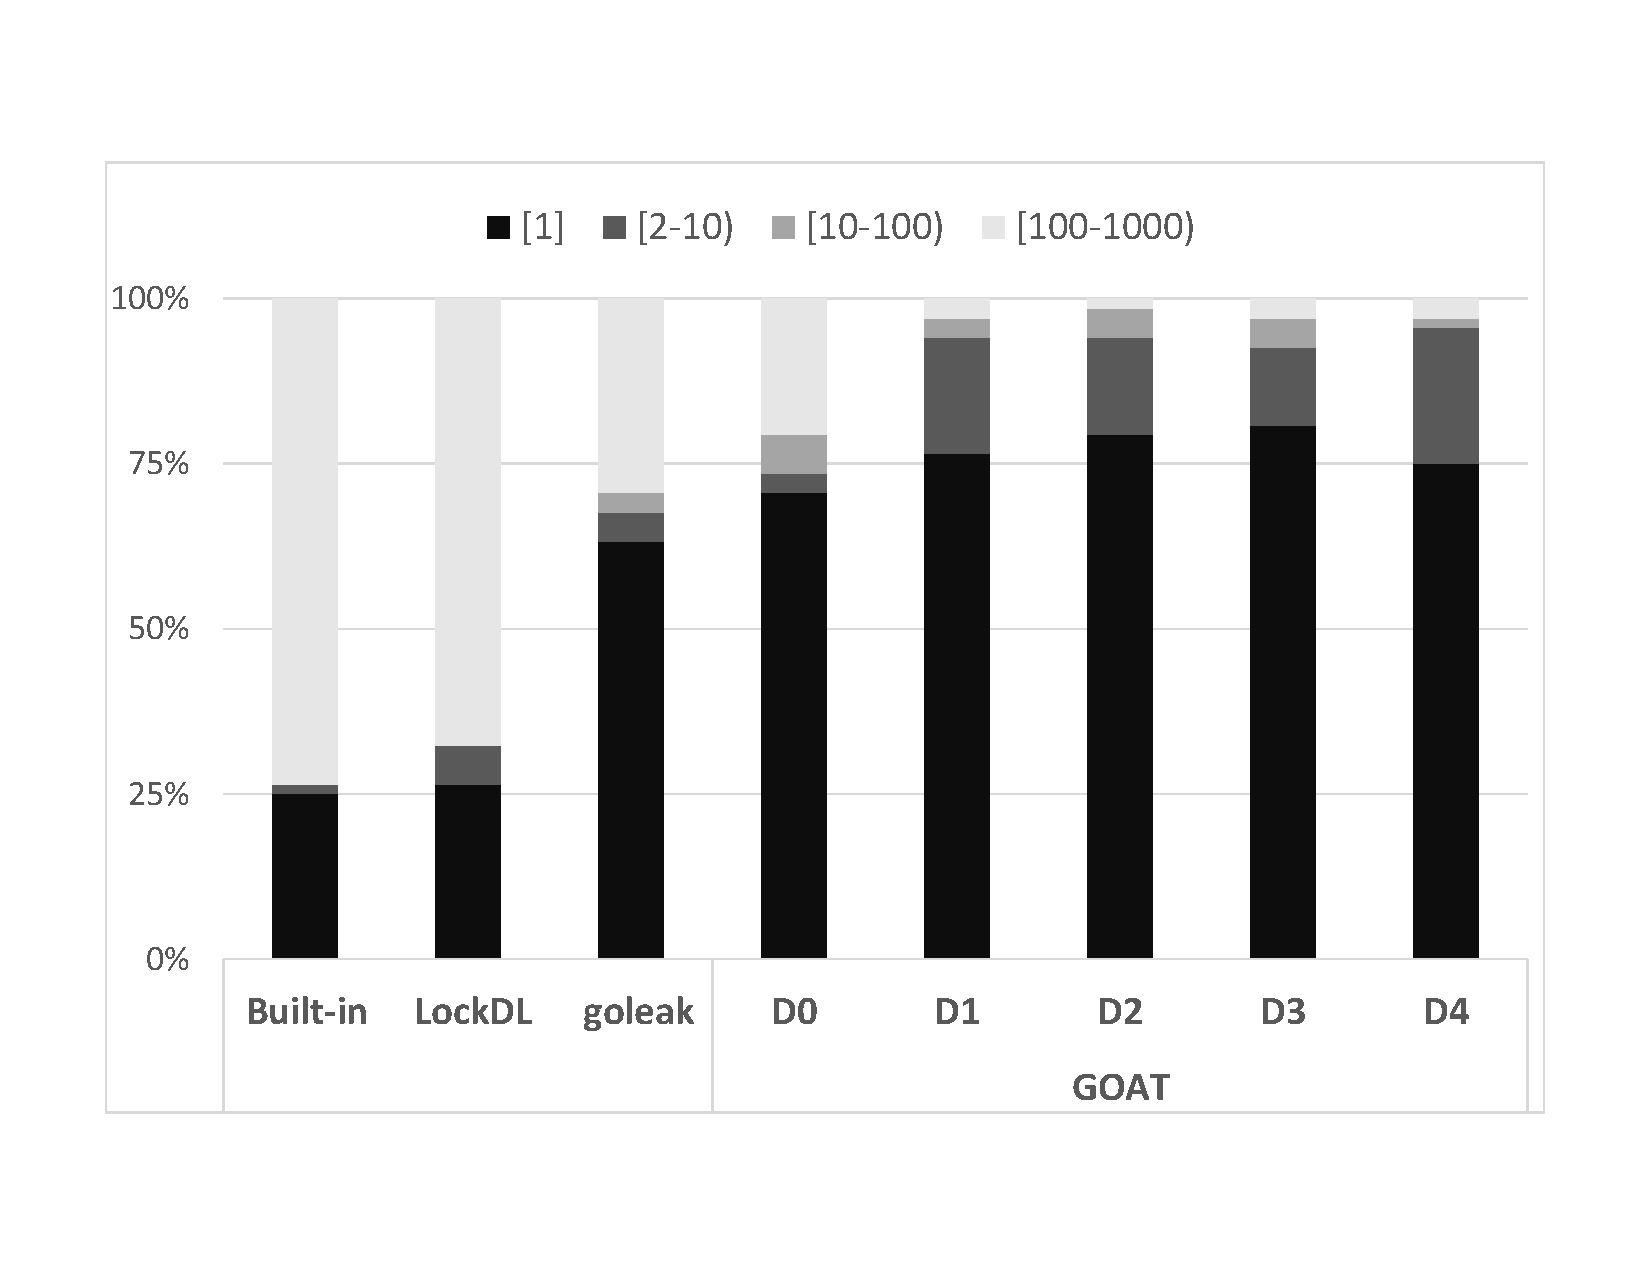
\includegraphics[width=.95\linewidth]{figs/P4_runs.pdf}
  \caption{Distribution of required number of iterations to detect the bug for each tool}
  \label{fig:runs}
\end{figure}
